%
% wiener.tex
%
% (c) 2020 Prof Dr Andreas Müller, Hochschule Rapperswil
%
\section{Wiener-Filter
\label{section:wiener-filter}}
\kopfrechts{Wiener-Filter}
Ein ähnliches Problem findet man in der Übertragungstechnik.
Wir gehen davon aus, dass ein Übertragungskanal ein Signal abschwächt
und mit einem Rauschsignal überlagert.
Die Abschwächung können wir selbstverständlich wieder rückgängig
machen, dabei wird aber auch das Rauschen verstärkt, so dass das
verstärkte Signal wenig mit dem ursprünglichen Signal zu tun hat.
Je stärker das Rauschen ist, desto vorsichtiger müssen wir mit
der Verstärkung sein.
Es dürfte also einen optimalen Verstärkungsfaktor geben, der 
das ursprüngliche Signal zwar nicht vollständig wiederherstellt, 
aber doch auf eine Weise, dass der Fehler möglichst klein ist.

\subsection{Grundprinzip
\label{filter:wiener:subsection:grundprinzip}}
Eine mathematischere Formulierung dieser Aufgabe ist die folgende.

\begin{aufgabe}
Sei $X$ eine Zufallsvariable mit Varianz $\operatorname{X}=\sigma$,
die von einem Übertragungskanal um den Faktor $a$ gedämpft wird.
Zusätzlich wird ein Rauschsignal $N$ mit Varianz $\sigma_N^2$ überlagert,
$X$ und $N$ sind unabhängig.
Finde den Faktor $b$, mit dem das gestörte Signal $Y=aX+N$ verstärkt werden
muss, damit sich ein Signal ergibt, dessen Abweichung vom ursprünglichen Signal
minimale Varianz hat.
\end{aufgabe}

Die Abweichung des verstärkten Signals $bY$ von $X$ hat die Varianz
\begin{align*}
\operatorname{var}(bY-X)
&=
\operatorname{var}(b(aX+N)-X)
=
\operatorname{var}((ab-1)X+bN)
=
(ab-1)^2 \operatorname{var}(X) + b^2\operatorname{var}(N).
\end{align*}
Um das Minimum zu bestimmen, leiten wir nach $b$ ab
\begin{align*}
0
&=
\frac{\partial}{\partial b} \operatorname{var}(bY-X)
=
2(ab-1)a \operatorname{var}(X) +2b\operatorname{var}(N)
\\
0&=
b(a^2\sigma^2 + \sigma_N^2) - a\sigma^2
\qquad\Rightarrow\qquad
b
=
\frac{a\sigma^2}{a^2\sigma^2+\sigma_N^2}
=
\frac{a}{a^2+\sigma_N^2/\sigma^2}.
\end{align*}
Diese Formel lässt sich auch leicht plausibilisieren.
Falls kein Rauschen vorhanden ist, also $\sigma_N=0$, dann kann
man für $b$ den Faktor $1/a$ verwenden, der die Abschwächung
vollständig rückgängig macht.
Falls das Rauschen im Vergleich zum Signal sehr gross ist, wird
$b\simeq 0$, es ist also gar nicht möglich, das Signal sinnvoll
wiederherzustellen.

Die Varianz des vestärkten Signals lässt sich jetzt ebenfalls
ausrechnen.
Sie ist
\begin{align*}
\operatorname{var}(bY-X)
&=
\biggl(\frac{a^2}{a^2+\sigma_N^2/\sigma^2}-1\biggr)^2\sigma^2
+
\biggl(\frac{a}{a^2+\sigma_N^2/\sigma^2}\biggr)^2 \sigma_N^2
\\
&=
\frac{\sigma_N^4/\sigma^2}{(a^2+\sigma_N^2/\sigma^2)^2}
+
\frac{a^2\sigma_N^2}{(a^2+\sigma_N^2/\sigma^2)^2}
=
\sigma_N^2\frac{a^2+\sigma_N^2/\sigma^2}{(a^2+\sigma_N^2/\sigma^2)^2}
\\
&=
\frac{\sigma_N^2}{a^2+\sigma_N^2/\sigma^2}.
\end{align*}
Auch diese Formel ist intuitiv nachvollziehbar.
Falls kein Rauschen vorhanden ist, also $\sigma_N=0$, ist die Rekonstruktion
ohne Fehler möglich.
Je grösser das Rauschen wird, desto grösser wird auch der Fehler.
Wenn das Rauschen viel stärker ist als das Signal,
also $\sigma_N^2 \gg \sigma^2$, dann ist der Summand $a^2$ im
Nenner vernachlässigbar und die Varianz strebt gegen $\sigma^2$,


Wir fassen dieses Resultat im folgenden Satz zusammen.

\begin{satz}[Wiener]
\label{filter:wiener:primitiv}
Wir ein Signal $X$ mit Varianz $\sigma^2$ um den Faktor $a$ abgeschwächt
und von einem unabhängigen Rauschsignal $N$ mit Varianz $\sigma_N^2$
überlagert, dann kann aus $Y=aX+N$ das ursprüngliche Signal durch
Vestärkung mit dem Verstärkungsfaktor
\[
b=\frac{a}{a^2 + \displaystyle\frac{\sigma_N^2}{\sigma^2}}
\]
optimal wiederhergestellt werden in dem Sinn, dass die Varianz
von $bY-X$ minimal ist und den Wert
\[
\operatorname{var}(bY-X)
=
\frac{\sigma_N^2}{a^2+\sigma_N^2/\sigma^2}.
\]
hat.
\end{satz}


\subsection{Spektrale Filterung
\label{filter:wiener:subsection:spektral}}
Das grundlegende Filter-Prinzip von Satz~\ref{filter:wiener:primitiv}
ist zwar grundsätzlich anwendbar und wir werden den Formeln in
Abschnitt~\ref{filter:section:einfuerung} in einer praktischen 
Anwendung wieder begegnen.

In einem realen Übertragungskanal wird natürlich kein konstantes Signal
übermittelt,
vielmehr ist der Wert $X$ von der Zeit abhängig.
Auch werden von einem realen Übertragungskanal nicht alle Frequenzen
im gleichen Mass abgeschwächt, die Annahme eines einzigen, für alle
Frequenzen gleichermassen gültigen Faktors $a$ ist daher unrealistisch.
Ziel dieses Abschnitts ist daher die Entwicklung einer Verallgemeinerung
des Filterprinzips~\ref{filter:wiener:primitiv} für ein zeitabhängiges
Signal $X(t)$.

Sei also $X(t)$ ein beliebiges zeitabhängiges Signal mit $t\in\mathbb [0,2\pi]$.
Der Einfachheit halber nehmen wir an, dass der Erwartungswert von $X(t)$
verschwindet, also
\[
E(X)
=
\frac{1}{2\pi}\int_{-\infty}^\infty X(t)\,dt
=
0.
\]
Ein solches Signal kann man als Fourier-Reihe darstellen, die wir in der
komplexen Form
\[
X(t)
=
\sum_{k=-\infty}^\infty c_k e^{ik t}
\]
schreiben.
Wir nehmen an, dass sich die Wirkung des Übertragungskanals auf das
Signal dadurch beschreiben lässt, wie die einzelnen Koeffizienten
$c_k$ abgeschwächt werden.
Wir nehmen also an, dass das modifizierte Signal $GX(t)$ die Fourier-Reihe
\[
GX(t)
=
\sum_{k=-\infty}^\infty g_kc_k e^{ikt}
\]
hat.
$G$ ist ein linearer Operator auf zeitabhängigen Signalen.
Zusätzlich wird dem Signal jetzt noch ein unkorreliertes Störsignal
$N(t)$ überlagert, welches die Fourier-Reihe 
\[
N(t) = \sum_{k=-\infty}^\infty n_ke^{ikt}
\]
hat.
Auch hier nehmen wir der Einfachheit halber an, dass der Erwartungswert
verschwindet.

Das Störsignal $N$ soll nicht mit $X(t)$ korreliert sein.

Die Aufgabe ist jetzt, das Signal $X(t)$ durch geeignetes Verstärken
der mit Verstärkungsfaktoren $h_k$ zu rekonstruieren zu
\[
Y(t)
=
\sum_{k=-\infty}^\infty h_k(g_kc_k + n_k)e^{ikt}
\]
derart, dass die Varianz von $Y(t)-X(t)$ minimal ist.
Auch diese Operation können wir als Operator
\[
H(GX(t) + N(t))
=
\sum_{k\in\mathbb Z} h_k(g_kc_k+n_k)e^{ikt}
\]
beschreiben.


Die Varianz kann als Skalarprodukt von Funktionen geschrieben werden:
\begin{align}
\operatorname{var}(X-Y)
&=
\int_0^{2\pi} |Y(t)-X(t)|^2\,dt
\notag
\\
&=
\int_0^{2\pi} (Y(t)-X(t)) \cdot \overline{(Y(t)-X(t))}\,dt
\notag
\\
&=
\langle Y(t)-X(t), Y(t)-X(t)\rangle
\notag
\\
&=
\langle H(GX(t) + N(t))- X(t), H(GX(t)+N(t))-X(t) \rangle
\notag
\\
&=
\langle (HG-I)X-HN, (HG-I)X-HN\rangle
\notag
\\
&=
\notag
\langle (HG-I)X,(HG-I)X\rangle
+
\langle HN,HN\rangle
\\
&\qquad
+
\langle (HG-I)X,HN\rangle
+
\langle HN,(HG-I)X\rangle
\intertext{%
Wir nehmen an, das Signal und Rauschen unabhängig sind, dass also die
letzten zwei Terme verschwinden.
Das Parseval-Theorem besagt, dass man diese Skalarprodukte auch mit
den Fourier-Koeffizienten berechnen kann:}
&=
\sum_{k\in\mathbb Z}
(|(h_kg_k-1)c_k|^2 + |h_kn_k|^2).
\label{wiener:spektral:summe}
\end{align}
Die Koeffizienten $h_k$ können offenbar unabhängig voneinander gewählt
werden, man muss also nur noch sicherstellen, dass jeder einzelne Term
der Summe~\eqref{wiener:spektral:summe} minimal wird.

Wir müssen jetzt das Problem lösen, $h_k$ so zu bestimmen, dass
der zugehörige Term in \eqref{wiener:spektral:summe} minimal wird.
Zur Vereinfachung lassen wir die Indizes $k$ weg.
Wir brauchen das folgende Resultate

\begin{hilfssatz}
Seien $g,c,n\in\mathbb C$ gegeben.
Der Ausdruck
\[
Z = |(hg-1)c|^2 + |hn|^2
\]
wird minimiert durch 
\[
h = \frac{\overline{g}}{|g^2|+|n|^2/|c|^2}
\qquad\text{mit}\qquad
Z = \frac{|n|^2}{|g|^2 + |n|^2/|c|^2}.
\]
\end{hilfssatz}

\begin{proof}[Beweis]
Der Ausdruck $Z$ ist ein komplexes Skalarprodukt
\[
Z
=
\begin{pmatrix}
(hg-1)c&hn
\end{pmatrix}
\begin{pmatrix}
\overline{(hg-1)c}\\\overline{hn}
\end{pmatrix}.
\]
Das Minimum wird erreicht, wenn die Ableitung des ersten Faktors nach
$h$ einen Vektor liefert, der orthogonal ist zum zweiten:
\begin{align*}
0
=
\begin{pmatrix}
gc&n
\end{pmatrix}
\begin{pmatrix}
\overline{(hg-1)c}\\\overline{hn}
\end{pmatrix}
=
(\overline{h} |g|^2 - g )|c|^2
+
\overline{h} |n|^2
\quad&\Rightarrow\quad
\overline{h}(|g|^2|c|^2+|n|^2)=g|c|^2
\\
\quad&\Rightarrow\quad
h=\frac{\overline{g}}{|g|^2 + |n|^2/|c|^2}
\end{align*}
Durch Einsetzen dieses Wertes von $h$ in $Z$ erhält man
\[
Z
=
\biggl|
\frac{|g|^2}{|g|^2+|n|^2/|c|^2}
-1
\biggr|^2 |c|^2
+
\frac{|g|^2|n|^2}{(|g|^2+|n|^2/|c|^2)^2}
=
\frac{|n|^4/|c|^2 + |n|^2 |g|^2}{(|g|^2+|n|^2/|c|^2)^2}
=
\frac{|n|^2}{|g|^2+|n|^2/ |c|^2}.
\]
Damit ist alles bewiesen.
\end{proof}

Damit können wir jetzt den Wiener-Filter für ein beliebiges Signal
formulieren.

\begin{satz}[Wiener-Filter]
\label{filter:wiener:satz}
Sie $X(t)$ ein Signal mit Fourier-Koeffizienten $c_k$ und $N(t)$
ein von $X(t)$ unabhängiges Rauschen mit Fourier-Koeffizienten $n_k$.
Das Signal wird der Funktion $G(t)$ mit Fourier-Koeffizienten
$g_k$ gefaltet.
Eine im Sinne minimaler Varianz optimale Schätzung des gefalteten und
verrauschten Signals $Y(t) = G*X(t) + N(t)$ mit den Fourier-Koeffizienten
$y_k = g_kc_k+n_k$ wird durch 
\[
Z(t)
=
\sum_{k\in\mathbb Z}
\frac{\overline{g_k}}{|g_k|^2+|n_k|^2/|c_k|^2} y_k e^{ikt}
\]
gegeben.
\end{satz}

Viele Filter in der Praxis sind FIR-Filter und können daher genau
in der Form einer Faltung mit einer Funktion $G$ formuliert werden.
Auch ist das Rauschen $N(t)$ in der Praxis unvermeidlich.
Schon die Digitalisierung des Signals $G*X$ führt ein Rauschen von der
Grössenordnung eines Bits ein.
Dies reicht bereits, direkte Rekonstruktion des Signals $X(t)$ (siehe
Abschnitt~\ref{filter:wiener:subsection:deconvolution}) mit
Hilfe der Fourier-Theorie zu verunmöglichen.

%
% Entfaltung eines Signals
%
\subsection{Anwendung: Entfaltung
\label{filter:wiener:subsection:deconvolution}}
\begin{figure}
\centering
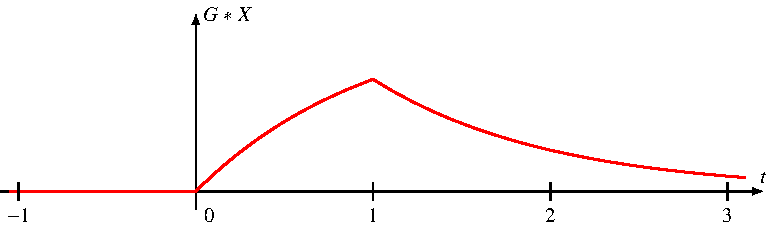
\includegraphics{8-filter/images/faltung.pdf}
\caption{Graph der Faltung von $G*X$ des Beispiels aus
Abschnitt~\ref{filter:wiener:subsection:deconvolution}
\label{filter:wiener:faltung:graph}}
\end{figure}
Als Beispiel für die Funktion des Wiener-Filters betrachten wir das Signal 
\[
X(t) = \begin{cases}
1&\quad 0\le t\le 1\\
0&\quad\text{sonst}
\end{cases}
\]
und falten es mit einer exponentiell abfallenden Impulsantwort
\[
G(t)
=
\begin{cases}
e^{-t}&\quad t \ge 0\\
0&\quad \text{sonst}
\end{cases}
\]
Die Ausführung der Faltung ergibt
\begin{equation}
X*G(t)
=
\begin{cases}
0&\quad t\le 0
\\[10pt]
\displaystyle
\int_0^t e^{\tau-t}\,d\tau
=
e^{-t}
\int_0^t e^{\tau}\,d\tau
=
e^{-t}[e^\tau]_0^t
=
e^{-t}(e^t-1)
=
1-e^{-t}
&\quad 0\le t\le 1
\\[10pt]
\displaystyle
\int_0^1 e^{\tau-t}\,d\tau
=
e^{-t}[e^\tau]_0^1
=
e^{-t}(e-1)
&\quad 1\le t
\end{cases}
\end{equation}
Das Signal $Y=G*X$ ist in Abbildung~\ref{filter:wiener:faltung:graph}
dargestellt, die steilen Flanken des ursprünglichen Rechteckimpulses
sind verloren gegangen.

Der Faltungssatz besagt, dass
$\mathcal{F}Y= \mathcal{F} (G*X) = \mathcal{F}G \cdot \mathcal{F}X$
ist.
Falls $\mathcal{F}G$ nirgends verschwindet, kann $X$ durch Division 
rekonstruiert werden:
\begin{equation}
\mathcal{F}X
=
\frac{\mathcal{F}Y}{\mathcal{F}G}
\quad\Rightarrow\quad
X=\mathcal{F}^{-1}
\frac{\mathcal{F}Y}{\mathcal{F}G}.
\label{filter:wiener:invertierung}
\end{equation}
Im Allgemeinen kann man aber nicht davon ausgehen, dass $\mathcal{F}G$
keine Nullstellen hat.
Die Funktionen $\mathcal{F}Y$ und $\mathcal{F}G$ müssen aber die gleichen 
Nullstellen haben.
Wenn die Nullstellen isoliert sind, kann die
Invertierung~\eqref{filter:wiener:invertierung} trotzdem funktionieren.

Zusätzlich wird dem Signal jetzt noch ein weisses Rauschen überlagert.
Jetzt kann man nicht mehr davon ausgehen, dass $\mathcal{F}Y$ und 
$\mathcal{F}G$ die gleichen Nullstellen haben, die 
Invertierung~\eqref{filter:wiener:invertierung} kann also nicht
mehr funktionieren.

Die Fouriertransformation von $G(t)$ ist
\begin{equation}
\mathcal{F}G(k)
=
\hat{G}(k)
=
\int_0^\infty e^{-t} e^{ikt}\,dt
=
\int_0^\infty e^{(ik-1)t}\,dt
=
\biggl[\frac{1}{ik-1}e^{ik-1}\biggr]_0^\infty
=
\frac{1}{1-ik}.
\end{equation}
Im vorliegenden Fall verschwindet $\mathcal{F}G$ nirgends, aber
für $k\to\infty$ geht $\mathcal{F}G(k)$ gegen $0$.
Die Fouriertransformation des überlagerten Rauschens ist dagegen überall
unter gleich gross, der Quotient $\hat{N}/\hat{G}$ wird also für
grosse $k$ über alle Grenzen wachsen.
Es ist daher notwendig, den Wiener-Filter anzuwenden.

Nach der allgemeinen Theorie muss zur approximativen Rekonstruktion
von $X$ aus $Y=G*X+N$ die Fourier-Transformierte von $Y$ statt mit
$1/\hat{G}$ mit
\[
\frac{\overline{\hat{G}(k)}}{
|\hat{G}(k)|^2
+
|\hat{N}(k)|^2/|\hat{X}(k)|^2
}
=
\frac{1/(1+ik)}{
1/(1+k^2)
+
|\hat{N}(k)|^2/|\hat{X}(k)|^2
}
=
\frac{1-ik}{1+(1+k^2) |\hat{N}(k)|^2/|\hat{X}(k)|^2}
\]
multipliziert werden.

Im vorliegenden Beispiel $\hat{X}$ zwar bekannt, aber im Allgemeinen
kann man nur davon ausgehen, eine ungefähre Grössenordnung für das
Verhältnis $|\hat{N}(k)|/\hat{X}(k)|$ von Rauschen zum Signal
zu kennen.
Für ein weisses Rauschen können wir zum Beispiel annehmen, das $\hat{N}(k)$
für alle $k$ ungefähr gleich gross ist.
Wir können daher das Verhältnis von Rauschen zum Signal durch einen
konstanten Wert $n$ ersetzen.
Der Korrekturfaktor des Wiener-Filters wird damit
\[
\frac{1-ik}{1+(1+k^2) s},
\]
wobei $s$ ein Parameter ist, mit dem die Leistung des Filters gesteuert
werden kann.

\begin{figure}
\centering
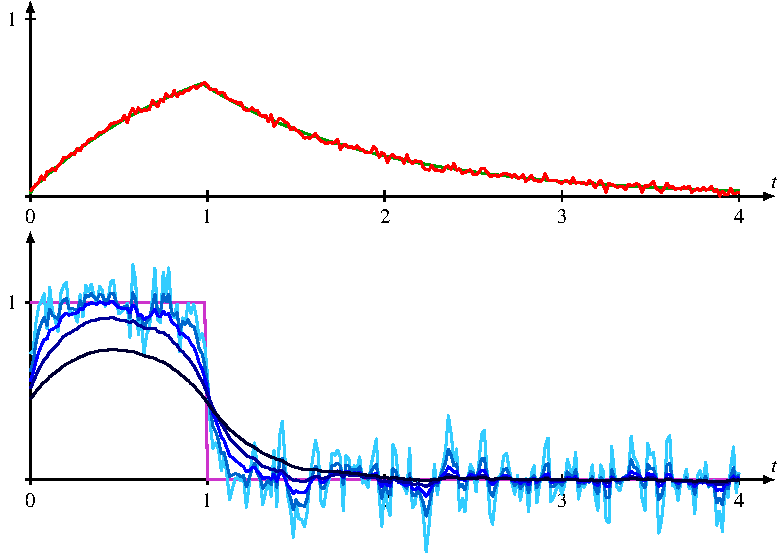
\includegraphics{8-filter/images/filterung.pdf}
\caption{Entfaltung am Beispiel der Funktionen in
Abschnitt~\ref{filter:wiener:subsection:deconvolution}.
In der oberen Abbildung das gefaltete Signal $G*X$ in grün,
das verrauschte Signal $G*X+N$ in rot.
In der unteren Abbildung die Rekonstruktion des Signals ohne
Rauschen (pink) und die Rekonstruktion des verrauschten Signals
mit Hilfe des Wiener-Filters mit verschiedenen angenommen
Werten von $|\hat{N}|^2/|\hat{X}^2|$ in blau.
\label{filter:wiener:rekonstruktion}}
\end{figure}
In Abbildung~\ref{filter:wiener:rekonstruktion} ist oben das 
gefaltete Signal $G*X$ grün dargestellt und rot das gleiche Signal
mit überlagertem Rauschen.
Im unteren Graphen ist in pink die Rekonstruktion des unverrauschten
Signals mit Hilfe der Fourier-Theorie dargestellt.
In verschiedenen Blautönen ist die Rekonstruktion des verrauschten
Signals mit Hilfe des Wiener-Filters für verschiedene angenommene
Werte von $|\hat{N}|^2/|\hat{X}|^2$ oder gleichwertig verschiedene
Werte des Parameters $s$ dargestellt.
Für grosse Werte des Parameters $s$ wird das Rauschen zwar sehr stark
reduziert, aber die steilen Flanken des Signals können auch nicht
wiederhergestellt werden.

\subsection{Anwendung: Bildverbesserung mit Wiener-Filter
\label{filter:wiener:subsection:bildverbesserung}}
\begin{figure}
\centering
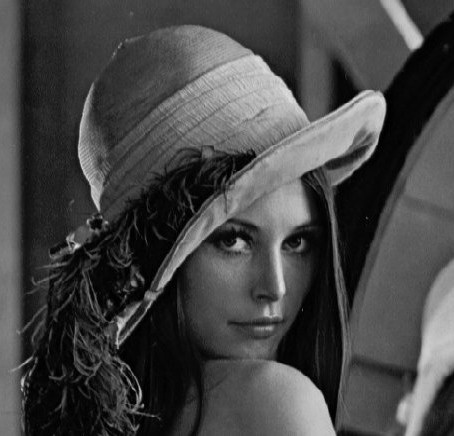
\includegraphics[width=0.48\hsize]{8-filter/images/lena.jpg}
\quad

\includegraphics[width=0.48\hsize]{8-filter/images/lena-noisy.png}
\caption{Originalbild und mit einer Gaussfunktion verschmiertes Bild.
Durch die Rundung auf ganzzahlige Pixelwerte im Interval $[0,255]$
nach der Faltung mit der Gaussfunktion wird für das Auge nicht
sichtbares Quantisierungsrauschen hinzugefügt, welches bereits die
exakte Wiederherstellung des Bildes verunmöglicht.
\label{filter:wiener:figure:faltung}}
\end{figure}
\begin{figure}
\centering
\includegraphics[width=\hsize]{8-filter/images/deconvolution.pdf}
\caption{Wiederherstellung des Bildes mit Hilfe des Wiener-Filters.
Das Quantisierungsrauschen verunmöglicht die exakte Wiederherstellung,
die für sehr kleinem Parameterwert ganz links oben erwartet wird.
Sehr grosse Werte von $K$ dämpfen die hohen Frequenzen wieder dermassen
stark, dass die Kanten wieder unscharf werden.
\label{filter:wiener:figure:wiederherstellung}}
\end{figure}
Die optische Abbildung einer Szene führt zu Verlusten zum Beispiel
durch Unzulänglichkeiten der Optik oder ungenügende Scharfstellung.
Die Wellennatur des Lichtes und die daraus resultierende
Beugung führt zu einer unvermeidlichen Beschränkung der Auflösung.
Die Digitalisierung des Bildes durch den Bildsensor führt zusätzliches,
zufälliges Rauschen ein.
Es stellt sich die Frage, ob uns die genaue Kenntnis des Objektivs und der
Verteilung des Rauschens in die Lage versetzt, das Bild möglichst
gut zu rekonstruieren.

Mathematisch können Bilder als Funktionen $f(x,y)$ von Pixelkoordinaten 
betrachtet werden.
Die Bildveränderungen bei der Abbildung können als Faltung mit der sogenannten
point spread function $G(x,y)$ beschrieben werden.
Zum Beispiel führt die Faltung mit der gausssche Funktion
\[
G(x,y) = \frac{1}{2\pi\sigma^2} e^{-(x^2+y^2)/2\sigma^2}
\]
zu einem unscharfen Bild, wie in Abbildung~\ref{filter:wiener:figure:faltung}
dargestellt.
Das Faltungstheorem für Funktionen in der Ebene besagt, dass die
zweidimensionale Fourier-Transformation die Faltung in ein punktweises
Produkt verwandelt.
Der Wiener-Filter nach Satz~\ref{filter:wiener:satz} gilt daher sinngemäss
auch für Bilder.

Um den Wiener-Filter anzuwenden, muss man Informationen über die spektrale
Verteilung des Rauschens haben, also die Koeffizienten $n_k$ kennen.
Oft genügt es, eine Schätzung für das Verhältnis zwischen Rauschen und
Signal zu verwenden.
Zum Beispiel führt die Rundung von Pixelwerten auf ganzzahlige Werte im
Interval $[0,255]$ zu unvermeidlichem Quantisierungsrauschen mit einer
Varianz der Grössenordnung $1/(256^2)\simeq 10^{-5}$.
Oft enthalten Bilder grosse Gebiete gleicher Helligkeit.
Die einzige Variabilität innerhalb solcher Gebiet stammt vom Rauschen her.
Die Varianz der Pixelwerte in einem solche Gebiet ist daher eine gute
Schätzung für das Rauschen.

Ausserdem muss man Informationen über die point spread function $G$ haben.
Enthält die abgebildete Szene isolierte helle Punkte, wie dies in der
Astrophotographie üblicherweise der Fall ist, dann ist das Bild
eines solchen Punktes ein guter Ausgangspunkt für die Funktion $G$.
Manchmal lässt sich eine gute Hypothese für die point spread function
aus theoretischen Überlegungen ableiten.
Ein unscharf eingestelltes Objektiv kann zum Beispiel als Faltung mit
einer Kreisscheibe, auch bekannt als {\em Bokeh}, modellieren.
Luftunruhe führt dagegen zu einer point spread function, die gut
von einer Gauss-Funktion wiedergeben wird.

Die Wirkung des Wiener-Filters ist in den
Abbildungen~\ref{filter:wiener:figure:faltung} und
\ref{filter:wiener:figure:wiederherstellung} dargestellt.
In Abbildung~\ref{filter:wiener:figure:faltung} wird ein Bild
mit einer Gaussfunktion gefaltet, was zu einem unscharfen Bild führt.
Nicht erkannbar im rechten Bild in Abbildung~\ref{filter:wiener:figure:faltung}
ist das Quantisierungsrauschen, welches bei der Umwandlung der
reellen Werte der Faltung in ganzzahlige Pixelwerte entsteht.
Diese für das blosse Auge nicht erkennbare Rauschen ist bereits
genug, die Rekonstruktion des Bildes zu verunmöglichen.

In Abbildung~\ref{filter:wiener:figure:wiederherstellung}
wird der Wiener-Filter mit verschiedenen von $k$ unabhängigen Werten
$K$ für $|n_k|^2/|c_k|^2$ auf das unscharfe Bild von
Abbildung~\ref{filter:wiener:figure:faltung} angewendet.
Zu kleine Werte von $K$ führen zu einem nicht erkennbaren Bild, die
hochfrequenten Komponenten des Bildes und vor allem des Rauschens
sind derart verstärkt worden, dass das ursprüngliche Bild wiedergefunden
werden kann.
Zu grosse Werte von $K$ führen kaum zu einer Verbesserung des Bildes.
Es wird vor allem das Rauschen reduziert, welches ohnehin nicht
erkennbar war.









